\documentclass[]{aa}

\usepackage{txfonts}
\usepackage{ulem}
\usepackage{amsmath, mathtools}
\usepackage[colorlinks,breaklinks]{hyperref}
\hypersetup{linkcolor=blue,citecolor=blue,filecolor=black,urlcolor=blue}

\newcommand{\orcid}[1]{
\href{https://orcid.org/#1}{

\includegraphics[height=11pt]{General_figures/ORCIDiD_icon128x128.png}}}

\def\l{\lambda}\def\L{\Lambda}

\newcommand{\nn}[1]{\textcolor[rgb]{1.0, 0.6, 0.0}{#1}}
\newcommand{\mr}[1]{\textcolor[rgb]{0.5, 0.20, 0.3}{#1}}
\newcommand{\yc}[1]{\textcolor[RGB]{217, 22, 102}{#1}}
\newcommand{\prob}[2]{\mathcal{P}\left( #1 \mid #2\right)}

\begin{document}
\title{Redshift Evolution of the Underlying Type Ia Supernova Stretch
Distribution}

\author{
    N. Nicolas \thanks{n.nicolas@ip2i.in2p3.fr, equal contribution} \inst{1} 
    \and M. Rigault \thanks{m.rigault@ip2i.in2p3.fr, equal contribution} \inst{1}
    \orcid{0000-0002-8121-2560}
    \and\\ Y. Copin \inst{1}
    \orcid{0000-0002-5317-7518}
    \and R. Graziani \inst{2}
    \and G. Aldering\inst{3}
    \and M. Briday\inst{1}
    \and Y.-L. Kim\inst{1}
    \orcid{0000-0002-1031-0796}
    \and J. Nordin\inst{4}
    \and Saul Perlmutter\inst{3}
    \and M. Smith\inst{1,5}
    \orcid{0000-0002-3321-1432}
}

\institute{Université de Lyon, F-69622, Lyon, France; Université de Lyon
    1, Villeurbanne; CNRS/IN2P3, Institut de Physique des Deux Infinis, Lyon
    \and 
    Université Clermont Auvergne, CNRS/IN2P3, Laboratoire de
    Physique de Clermont, F-63000 Clermont-Ferrand, France.
    \and
    Physics Division, Lawrence Berkeley National Laboratory, 
    1 Cyclotron Road, Berkeley, CA, 94720 
    \and
    Institut fur Physik, Humboldt-Universität zu Berlin, Newtonstr. 15,
    12489 Berlin
    \and
    University of Southampton: Southampton, GB
}

\date{Submitted to A\&A the 19th of May 2020}

\abstract{The true nature of type Ia supernovae (SNe~Ia) remains largely
    unknown, and as survey statistics increase, the question of astrophysical
    systematic uncertainties rises, notably that of the SN~Ia population
    evolution. In this paper, we study the dependence with redshift of the SN~Ia
    \texttt{SALT2.4} lightcurve stretch, a purely intrinsic SN property, to
    probe its potential redshift drift. The SN stretch has been shown to
    strongly correlate with the SN environment, notably with stellar age
    tracers. We model the underlying stretch distribution as a function of
    redshift, using the evolution of the fraction of young and old SNe~Ia as
    predicted by \cite{rigault2020}, and assuming constant underlying stretch
    distribution for each age population \textbf{consisting} of Gaussian
    mixtures. We test our prediction against published samples \textbf{cut} to
    have marginal magnitude selection effects, so that any observed change is
    indeed of astrophysical and not observational origin. \textbf{In this first
    study, there are indications} that the underlying SN~Ia stretch distribution
    is evolving as a function of redshift, and that the young/old drifting model
    is a better description of the data than any time-constant model, including
    the sample-based asymmetric distributions usually used to correct Malmquist
    bias. The favored underlying stretch model is the bimodal one derived from
    \cite{rigault2020}, \textbf{composed of} a high-stretch mode shared by both
    young and old environments, and a low-stretch mode exclusive to old
    environments. The precise impact of the redshift evolution of the SN Ia
    population intrinsic properties on cosmology remains to be studied. Yet, the
    astrophysical drift of the SN stretch distribution does affect current
    Malmquist bias corrections and thereby distances derived from SN affected by
selection effects. We highlight that such a bias will increase with surveys
covering increasingly larger redshift ranges, which is particularly important
for LSST.}

\keywords{Cosmology -- Type Ia Supernova -- Systematic uncertainties}
\maketitle

\section{Introduction}

Type Ia supernovae (SNe Ia) are powerful cosmological distance indicators that
have enabled the discovery of the acceleration of the Universe's expansion
\citep{riess1998, perlmutter1999}. They remain today a key cosmological probe to
understand the properties of dark energy (DE) as it is the only tool able to
precisely map the recent expansion rate ($z<0.5$), when DE is driving it
\citep[e.g.][]{scolnicastro2020}. They also are key to directly measure the
Hubble Constant ($H_0$), provided one can calibrate their absolute magnitude
\citep{riess2016, freedman2019}. Interestingly, the value of $H_0$ derived when
the SNe~Ia are anchored on Cepheids \citep[the SH0ES project,][]{riess2009,
riess2016} is $\sim5\sigma$ higher than what is predicted from cosmic microwave
background (CMB) data measured by Planck assuming the standard $\L$CDM
\citep{planck2018, riess2019, reid2019}, or when the SN luminosity is anchored
at intermediate redshift by the baryon acoustic oscillation (BAO) scale
\citep{feeney2019}. While using the tip of the red giant branch technique in
place of the Cepheids seem to favor an intermediate value of $H_0$
\citep{freedman2019, freedman2020}, time delay measurements from strong lensing
seem to also favor high $H_0$ values \citep{wong2019}.

The $H_0$ tension has received a lot of attention, as it could be a sign of new
fundamental physics. Yet, no simple solution is able to accommodate this $H_0$
tension when accounting for all other probes \citep{knox2019}, but see e.g.
\cite{poulin2019}. Alternatively, systematic effects affecting one or several
of the aforementioned analyses could also explain the tension.
\cite{rigault2015} suggested that SNe Ia from the Cepheid calibrator sample
differ by construction from the Hubble flow sample ones as the former
strongly favors young stellar populations, while the latter not. This
selection effect would impact the derivation of $H_0$ if SNe~Ia from young and
older environments differ in average standardized magnitudes. 

For the last decades, numerous analyses have studied the relation between SNe~Ia
and host properties, finding first that the standardized SNe~Ia magnitude
significantly depends on the host stellar mass, SNe~Ia from high-mass host being
brighter on average \cite[e.g.][]{kelly2010, sullivan2010, childress2013,
betoule2014, rigault2020, kim19}. This mass-step correction is currently used in
cosmological analyses \citep[e.g.][]{betoule2014, scolnic2018a}, including for
deriving $H_0$ \citep{riess2016, riess2019}. Yet, the underlying connection
between the SNe and their host remains unclear when using global properties such
as the host stellar mass, which raises the question of the accuracy of the
correction. More recently, studies have used the local SN environment to probe
more direct connections between the SN and its environments \citep{rigault2013},
showing that local age tracers such as the Local specific Star Formation Rate
(LsSFR) or the local color are more strongly correlated with the standardized SN
magnitude \citep{rigault2020, roman2018, kim18}, suggesting age as the driving
parameter underlying the mass-step. If true, this would have a significant
impact for cosmology, since the environmental correction to apply to SN
standardization could strongly vary with redshift. \citep{rigault2013,
childress2014, scolnic2018a}. Yet, the importance of local SN environmental
studies remains highly debated \cite[e.g.][]{jones2015, jones2019} and
especially the impact of such an astrophysical bias has on the derivation of
$H_0$ \citep{jones2015, riess2016, riess2018, rose2019}. 

The concept of the SN~Ia age dichotomy arose with the study of the SN~Ia rate.
\cite{mannucci2005, scannapieco2005, sullivan2006, aubourg2008} have shown that
the relative SNe~Ia rate in galaxies could be explained if two populations
existed, one young, following the host star formation activity, and one old
following the host stellar mass (the so called ``prompt and delayed'' or ``A+B''
model). In \cite{rigault2020} we used the LsSFR to classify which are the
younger (those with a high LsSFR) and which are the older (those with low
LsSFR). Furthermore, since the first SNe~Ia host analyses, the SN stretch has
been known to be strongly correlated with the SN host properties
\citep{hamuy1996, hamuy2000}, correlation that has been extensively confirmed
since \citep[e.g.][]{neill2009, sullivan2010, lampeitl2010, kelly2010,
gupta2011, dandrea2011, childress2013, rigault2013, pan2014, kim19}. Following
the ``A+B'' model and the connection between SN stretch and host properties,
\cite{howell2007} first discussed the potential redshift drift of the SN stretch
distribution. In this paper we revisit this analysis with the most recent SNe~Ia
dataset.

In this paper, we take a step aside to probe the validity of our modeling of the
SN population, which we claim to be constituted of two age-populations
\citep{rigault2013,rigault2015,rigault2020}: one old and one younger, the former
having on average lower lightcurve stretches and being brighter after
standardization. We use the correlation between the SN age, as probed by the
LsSFR, and the SN stretch to model the expected evolution of the underlying SN
stretch distribution as a function of redshift. This modeling relies on three
assumptions: (1) there are two distinct populations of SNe~Ia; (2) the relative
fraction of each of these populations as a function of redshift follows the
model presented in \cite{rigault2020} and (3) the underlying distribution of
stretch for each age sample is constant. This paper aims at testing this
specific model with datasets from the literature. Note that the progenitor age
as traced by the LsSFR seems to capture physical feature intrinsic to the
progenitor and/or explosion mechanism that the stretch alone is not capturing
\citep{nordin2018}.

We present in Section~\ref{sec:sample} the sample we are using for this
analysis, derived from the Pantheon catalog \citep{scolnic2018a}. We discuss the
importance of obtaining a ``complete'' sample, i.e.\ representative of the true
underlying SNe Ia distribution, and how we build one from the Pantheon sample.
We then present in Section~\ref{sec:modeling} our modeling of the distribution
of stretch and our results are presented in Section~\ref{sec:results}. In this
section we test whether the SN stretch distribution evolves as a function of
redshift and if the aforementioned age model is in good agreement with this
evolution. We briefly discuss these results in the context of SN cosmology in
Section~\ref{sec:discussion} and we conclude in Section~\ref{sec:ccl}.

\section{Complete Sample Construction}\label{sec:sample}
\subsection{Applying redshift cuts}\label{ssec:cuts}

We base our analysis on the most recent comprehensive SNe~Ia compilation, the
Pantheon catalog from \cite{scolnic2018a}. A naive approach to test the SN
stretch redshift drift would be to simply compare the observed SN stretch
distributions in a few bins of redshift. In practice, however, differential
selection effects are affecting the observed SN stretch distributions. Indeed,
because the observed SN~Ia magnitude correlates with the lightcurve stretch (and
color), the first SNe~Ia that a magnitude-limited survey will miss are the
lowest-stretch (and reddest) ones. Consequently, if magnitude-related selection
effects are not accounted for, one might confuse true population drift with
survey properties, and conversely.

Assuming sufficient (and unbiased) spectroscopic follow-up for acquiring typing
and host redshift, the selection effects of magnitude-limited surveys should be
negligible below a given redshift at which even the faintest SNe~Ia can be
observed. \textbf{In practice such spectroscopic following has not always been
the norm as discussed below.} In contrast, targeted surveys have highly complex
selection functions and will be discarded from our analysis. Modern SN cosmology
samples such as the Pantheon one are now dominated by magnitude-limited surveys
\textbf{which have easier to model selection functions}.

We present in Fig.~\ref{fig:maglim} the lightcurve stretch and color of SNe~Ia
from the following surveys: PanStarrs \citep[PS1][]{rest2014}, the Sloan Digital
Sky Survey \citep[SDSS][]{frieman2008} and the SuperNovae Legacy Survey
\citep[SNLS][]{astier2006}. An ellipse in the \textsc{\texttt{SALT2.4}} $(x_1,
c)$ plane with $x_1 = \pm 3$ and $c = \pm 0.3$ encapsulates the full
distribution \citep{guy2007,betoule2014}; see also \citet{bazin2011} and
\citet{campbell2013} for similar contours, the second using a more conservative
$|c| \leq 0.2$ cut. Assuming the SN absolute magnitude with $x_1=0$ and $c=0$ is
$M_0=-19.36$ \citep{kessler2009,scolnic2014}, we can derive the absolute
standardized magnitude at maximum of light $M = M_0 - \alpha x_1 + \beta c$
along the aforementioned ellipse given the standardization coefficient
$\alpha=0.156$ and $\beta=3.14$ from \cite{scolnic2018a}: the faintest SN~Ia is
that with $(x_1=-1.65, c=0.25)$ and an absolute standardized magnitude at peak
in Bessel $B$ band of $M^{t_0}_{\min} = -18.31$~mag. Since one ought to detect
this object typically 5 days before and a week after peak to build a suitable
lightcurve, the effective limiting standardized absolute magnitude is
approximately $M_{\lim} = -18.00$~mag. Hence, given the magnitude limit
$m_{\lim}$ of a magnitude limited survey, one can derive the maximum redshift
$z_{\lim}$ above which the faintest SNe~Ia will be missed using the relation
between apparent magnitude, redshift and absolute magnitude $\mu(z_{\lim}) =
m_{\lim} - M_{\lim}$.

\begin{figure}
    \centering
    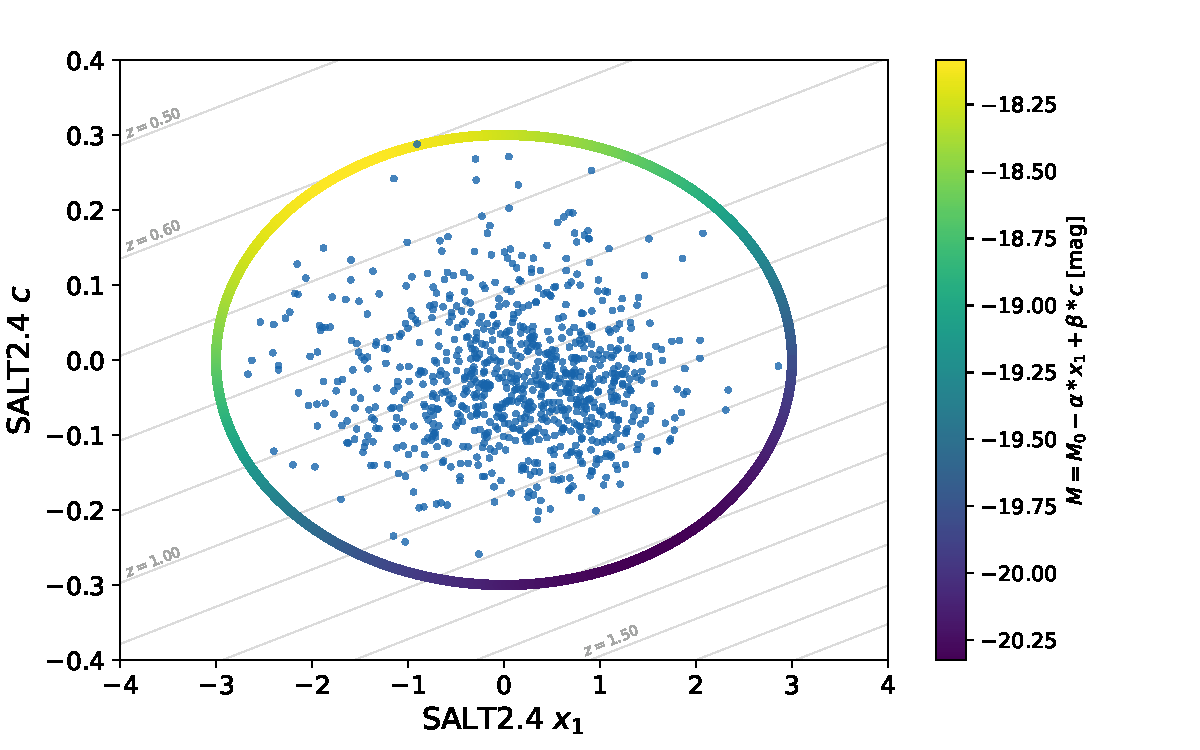
\includegraphics[width=0.95\linewidth]{Article_figures/zmax_maglim_snls.pdf}
    \caption{\textsc{\texttt{SALT2.4}} stretch ($x_1$) and color ($c$)
        lightcurve parameters of SNe~Ia from the SDSS, PS1 and SNLS samples of
        the Pantheon catalog. The individual SNe are shown as blue dots. The
        ellipse $(x_1=\pm3, c=\pm0.3)$ is displayed, colored by the
        corresponding standardized absolute magnitude using the $\alpha$ and
        $\beta$ coefficients from \cite{scolnic2018a}. The grey diagonal lines
        represent the $(x_1, c)$ evolution for $m = m_{\lim}$, for $z$ between
        $0.50$ and $z=1.70$ using SNLS's $m_{\lim}$ of $24.8$~mag.}
    \label{fig:maglim}
\end{figure}

\textbf{We will thus consider a set of cuts that will define a first fiducial
    sample, taking the limits as initially suggested by the previous
    completeness analysis. \textbf{However,} as this solution might be over
    simplistic to create a complete sample, e.g., for it ignores follow-up
    efficiency, we also consider another set of cuts to define a so-called
    conservative sample. This latter is smaller and therefore less statistically
    constraining, but also inherently less prone to selection effects. If the
    redshift drift is still significant in the conservative sample, it would be
    even more meaningful in a carefully-tailored selection-free sample. The goal
    of this study is to build the first implementation of a SN Ia properties
    drift modeling before refining it on a more complex, yet more accurate,
follow-up analysis also accounting for precise selection modeling using, e.g.,
the SNANA package \citep{SNANA}.}

SNLS typically acquired SNe~Ia in the redshift range $0.4<z<0.8$; at these
redshifts, the rest-frame Bessel $B$ band roughly corresponds to the SNLS $i$
filter, that has a $5\sigma$ depth of
24.8~mag\footnote{\href{https://www.cfht.hawaii.edu/Science/CFHTLS/cfhtlsfinalreleaseexecsummary.html}{CFHT
final release website.}}. This converts to a $z_{\lim}=0.60$, in agreement with
\cite{neill2006}, \cite{perrett2010} and \cite{bazin2011}. Fig.~14 of
\citet[][see their Section~5]{perrett2010} suggests however a lower limit of
$z_{\lim}=0.55$. \textbf{We will therefore use $z=0.60$ and $z=0.55$ as redshift
limits for the fiducial and conservative cuts, respectively.}

Similarly, PS1 observed SNe~Ia in the range $0.2<z<0.4$, their $g$-band
$5\sigma$ depth is 23.1~mag \citep{rest2014}, which yields $z_{\lim}=0.31$, in
agreement with, e.g., Fig.~6 of \cite{scolnic2018a}. \textbf{If we were to be
    conservative, this figure would also suggest of a more stringent
$z_{\lim}=0.27$ cut; hence, we will use $0.31$ and $0.27$ for our fiducial and
conservative cuts, respectively.}

In a similar redshift range, SDSS has a limiting magnitude of 22.5
\citep{dilday2008, sako2008}, which would lead to $z_{\lim}=0.24$. However, the
SDSS surveys \textbf{had to contend with limited spectroscopic resources. As
discussed in} \citet[][Section~2]{kessler2009}, during the first year of SDSS,
SNe~Ia with $r<20.5$~mag were favored for spectroscopic follow-up, corresponding
to a redshift cut at $0.15$. For the rest of the SDSS survey, additional
spectroscopic resources were available, and \cite{kessler2009} and
\cite{dilday2008} show a reasonable completeness up to $z_{\lim}=0.2$. Following
these analyses, \textbf{we will use $z_{\lim}=0.20$ and $z_{\lim}=0.15$ for our
fiducial and conservative cuts, respectively.}

The sample selection is summarized in Table~\ref{tab:sample}, and the redshift
distribution of these three surveys is shown in Fig.~\ref{fig:cuts}. As
expected, the selected redshift limits \textbf{are roughly located slightly
before the peak of these histograms. In Section 2.2 we validate that these
redshift limits are effective for constructing nearly volume-limited subsamples
from samples that were initially more closely magnitude-limited in their search
or spectroscopic follow-up.}

\begin{table}
    \centering
    \caption{Composition of the SNe~Ia dataset used in this analysis.
    Conservative cuts are indicated in parentheses. \textbf{The SNf limit is set by
\cite{rigault2020}, see text.}}
    \label{tab:sample}
    \begin{tabular}{l c c}
        \hline\hline
        Survey & $z_{\lim}$ & $N_{\mathrm{SN}}$ \\
        \hline
        SNf & 0.08 & 114 \\
        SDSS & 0.20 (0.15) & 167 (82)\\
        PS1 & 0.31 (0.27) & 160 (122)\\
        SNLS & 0.60 (0.55) & 102 (78)\\
        HST & -- & 26 \\
        \hline
        Total & -- & 569 (422) \\
        \hline
    \end{tabular}
\end{table}

\begin{figure}
    \centering
    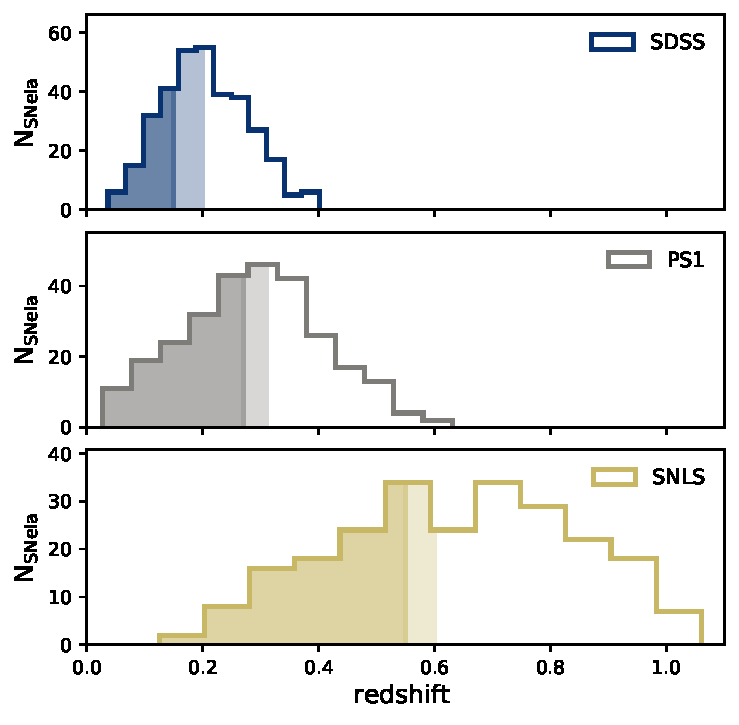
\includegraphics[width=0.95\linewidth]{Article_figures/hist_surveys_cuts_55-cividis.pdf}
    \caption{\textit{From top to bottom}: Redshift histograms of SNe~Ia from the
        SDSS, PS1 and SNLS dataset respectively (data from Pantheon,
        \citealt{scolnic2018a}). The colored parts represent the distribution of
        SNe~Ia kept in our analysis for they are supposedly free from selection
    bias (see Section~\ref{sec:sample}). The darker (resp. lighter) color
responds to the conservative (resp. fiducial) selection cut.}
    \label{fig:cuts}
\end{figure}

In addition, we use the SNe~Ia from the Nearby Supernova Factory
\citep[SNfactory,][]{aldering2002} published in \cite{rigault2020} and that have
been discovered from non-targeted searches (114 SNe~Ia, see their sections~3
and~4.2.2; SNe~Ia time series are published in \citealt{saunders2020}, see also
\citealt{aldering2020}). \textbf{For this dataset, spectroscopic screening was
    done for candidates with $r \lesssim 19.5$; redshift cuts were then applied
    when selecting which SN Ia to follow, resulting in a redshift range of $0.02
    < z < 0.09$, further reduced to $<0.08$ in \cite{rigault2020} for extracting
local host properties.} These 114 SNfactory SNe~Ia are thus in the
volume-limited part of the survey (Aldering et al., in prep.), and are therefore
assumed to be a random sampling of the underlying SN population. The SNfactory
sample is particularly useful for studying SN property drift, as it enables us
to have a large complete SN~Ia sample at $z<0.1$. 

Finally, we include the HST sample from Pantheon \citep{strolger04}.
\textbf{These high-redshift SNe are of great interest as they provide the
    greatest leverage for testing evolution. While at these redshifts the
    supernovae typing is challenging, the target classification was robust
    enough to include them within the cosmological analysis \citep{scolnic2018a}
    and we do not add further quality cuts. Section~\ref{sec:results} highlights
    that, while compatible with it, our results are not dependent on the
    inclusion of this dataset.}

We present the stretch distribution and redshift histogram of these five surveys
up to their respective $z_{\lim}$ in Fig.~\ref{fig:sample}. \textbf{We observe
that the fraction of low-stretch SNe (typically $x_1 < -1$) seems to decrease as
a function of redshift; this is confirmed in Fig.~\ref{fig:modelall} in which}
the evolution of the mean stretch is shown, \textbf{with} the data split in
redshift bins of regular sample size. We see that SNe~Ia at higher redshift have
on average larger stretch ($0.34 \pm 0.10$ at $z\sim0.65$) than those at lower
redshift ($-0.17\pm 0.10$ at $z\sim0.05$), suggesting that the underlying
stretch distribution is \textbf{evolving with redshift}.

\begin{figure}
    \centering
    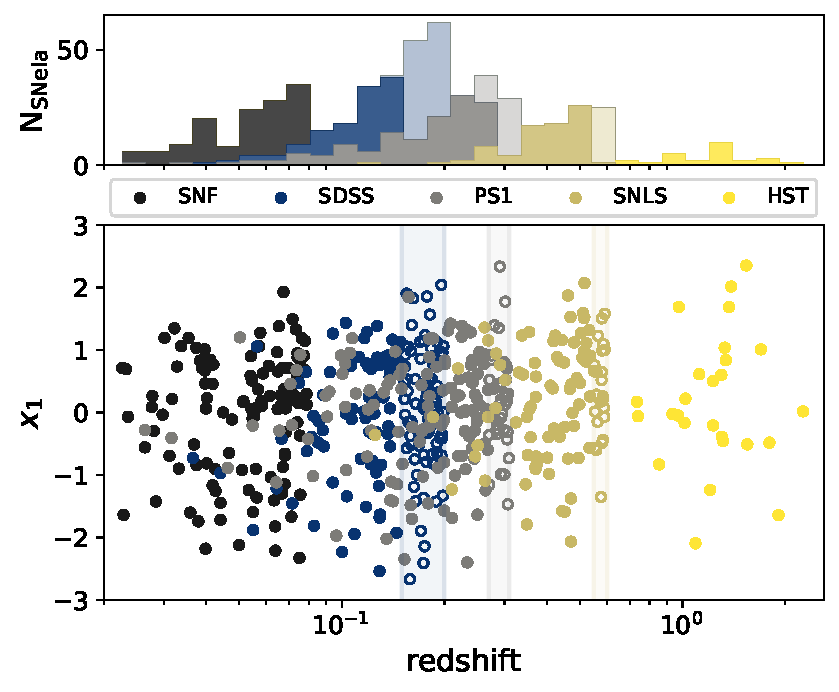
\includegraphics[width=0.95\linewidth]{Article_figures/stretchs-cut_btw_hist_stac_75-lb-cividis.pdf}
    \caption{\textit{Bottom:} \textsc{\texttt{SALT2.4}} lightcurve stretch as a
        function of redshift for each survey considered in this analysis (see
        legend). Solid (resp.\ open) markers correspond to the conservative
        (resp.\ fiducial) redshift cuts. \textit{Top:} stacked redshift
    histograms in dark (resp.\ light) colors for the conservative (resp. \
fiducial) redshift cuts.}
    \label{fig:sample}
\end{figure}

\subsection{Testing the construction of a volume-limited sample}\label{ssec:verify}

\textbf{In section~\ref{ssec:cuts}, we have built volume-limited samples from a
    set of magnitude-limited ones, using simple redshift cuts. This simplistic
    approach is statistically sub-optimal, but should be enough to demonstrate
    our key finding: a redshift evolution of stretch compatible with
    \cite{rigault2020} model. However, the possibility remains that a complex
    selection function related to follow-up efficiencies below our fiducial (or
    even conservative) cuts could still affect our sample, making it not fully
volume-limited; this would, in turn, bias our conclusion on the astrophysical
drift of the SNe~Ia population. We now look at this possibility.}

\textbf{To test for the existence of potential leftover selection biases in our
    sample, we compare the stretch and color distributions of the SNe~Ia
    originating from different datasets over overlapping redshift ranges: these
    distributions should be similar. Note that the redshift range has to be
    narrow enough so that any drift would be negligible.}

\textbf{The two samples that overlap the most in redshift are PS1 and SDSS in
    the redshift range $0.10 < z < 0.20$ (see Fig~\ref{fig:sample}). This
    corresponds to the 146 SNe~Ia from SDSS at the high redshift end and thus
    the most likely to be affected by residual selection effects (see the
    corresponding discussion in section~\ref{ssec:cuts}). Over that same
    redshift range, PS1 has 52 SNe~Ia, which are in the lowest redshift bins and
    thus unlikely to have any selection issue. To identify potential
    inconsistency between the PS1 and SDSS subsamples, Fig.~\ref{fig:distrib}
    (upper panels) compares the stretch and color distribution of both these
    surveys. The associated Kolmogorov-Smirnov (KS) similarity test $p$-values
are too high ($>10\%$) to conclude on any inconsistency, in agreement with the
visual impression from Fig.~\ref{fig:distrib}.}

\textbf{We perform a similar analysis for PS1 and SNLS over the redshift range
    $0.20 < z < 0.31$ (Fig.~\ref{fig:distrib}, lower panels), where the same
    conclusion can be drawn: there is no substantial sign of discrepancy in the
    stretch and color distributions between the low- and high-end of the SNLS
    and PS1 datasets, respectively. Nonetheless, the small size of the SNLS
    dataset at $z < 0.31$ (12 SNe~Ia vs. 90 for PS1) limits the sensitivity of
    the test, and only strong deviation would be noticeable. Extending the
redshift range to $0.20 < z < 0.40$ (though we have no PS1 data above 0.3)
allows to increase the SNLS subsample to 31, yet the stretch $p$-values remains
high (34\%) showing no sign of inconsistency.}

\begin{figure}
    \centering
    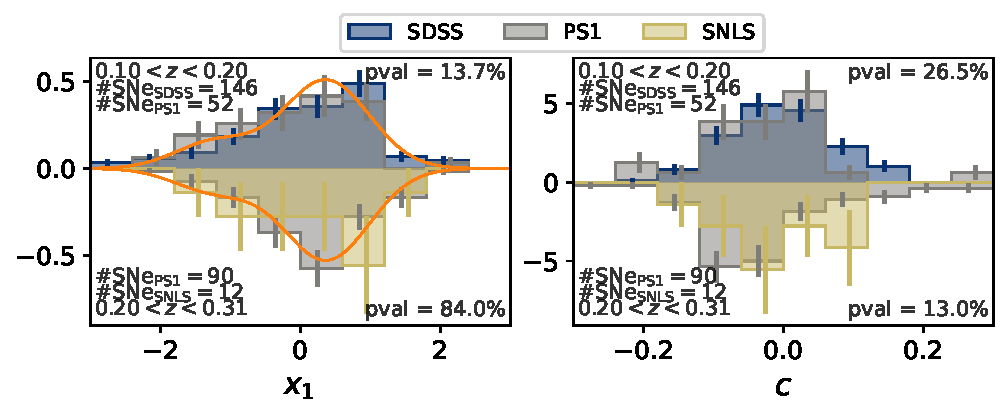
\includegraphics[width=0.95\linewidth]{Article_figures/both-cut_SDSS_SNLS_PS1.pdf}
    \caption{\textbf{$x_1$ (left) and $c$ (right) distribution histograms of
            different surveys overlapping in redshift. \textit{Facing up}: SDSS
            and PS1 within the redshift range $0.10 < z < 0.20$; \textit{facing
            down}: PS1 and SNLS within the redshift range $0.20 < z < 0.31$.
            Error bars show the Poisson noise. Our stretch ``Base'' model is
            illustrated in orange at the mean redshift of the redshift ranges,
            $0.15$ and $0.25$, respectively. Kolmogorov-Smirnov test $p$-values
            are indicated on the top (resp. bottom) of each panel showing no
            sign that the SDSS and PS1 (resp. PS1 and SNLS) $x_1$ and $c$
            distributions are not drawn from the same underlying
    distributions}}
    \label{fig:distrib}
\end{figure}

\textbf{We finally highlight that the SNe~Ia color is more prone to selection
    effects than stretch as illustrated in Fig.~\ref{fig:maglim}; see also e.g.,
    Fig.~3 of \cite{kessler2017}. Hence, since the comparison of color
    distributions shows no significant hint of leftover selection effect, it
    further supports our claim that our simple redshift-based selection criteria
    is sufficient to build a complete SNe~Ia sample required to test the
    redshift evolution of the stretch distribution.}

\section{Modeling the redshift drift}\label{sec:modeling}

\cite{rigault2020} presented a model for the evolution of the fraction of
younger and older SNe~Ia as a function of redshift following former work on
rates and delay time distributions \citep[e.g.,][]{mannucci2005,
scannapieco2005, sullivan2006, aubourg2008, childress2014, maozmannucci2014}.
In short, it was assumed that the number of ``young'' SNe~Ia follows the star
formation rate (SFR) in the Universe, while the number of ``old'' SNe~Ia follows
the number of Gyr-old stars in the Universe, i.e. the stellar mass (M$^*$).
Hence, if we denote $\delta(z)$ (resp. $\psi(z) = 1-\delta(z)$) the fraction of
young (resp. old) SNe~Ia in the Universe as a function of redshift, then the
ratio $\delta/\psi$ is expected to follow the evolution of the specific star
formation rate (SFR/M$^*$), which goes as $(1+z)^{2.8}$ until $z\sim2$
\citep[e.g.,][]{tasca2015}. Since $\delta(0.05) \sim \psi(0.05)$
\citep{rigault2013, rigault2020, wiseman2020}, in agreement with rate
expectations \citep{mannucci2006, rodney2014}, \cite{rigault2020} concluded that

\begin{equation}
    \label{eq:delta}
    \delta(z) = \left( K^{-1} \times (1+z)^{-2.8} +1 \right)^{-1}
\end{equation}
with $K=0.87$. This model is comparable to the evolution \textbf{subsequently}
predicted by \cite{childress2014} based on SN rates in galaxies depending on
their quenching time as a function of their stellar mass.

\subsection{``Base'' underlying stretch distribution}
\label{sec:basemodel}

To model the evolution of the full SN stretch distribution as a function of
redshift, given our aforementioned model of the evolution of the fraction of
younger and older SNe~Ia with cosmic time, we need to model the SN stretch
distribution for each age subsample. 

\cite{rigault2020} presented the relation between SN stretch and LsSFR
measurement, a progenitor age tracer, using the SNfactory sample. This relation
is shown in Fig.~\ref{fig:stretchlssfr} for the SNfactory SNe used in the
current analysis. Given the structure of the stretch-LsSFR scatter plot, our
model of the underlying SN~Ia stretch distribution is defined as follows:

\begin{figure*}
    \centering
    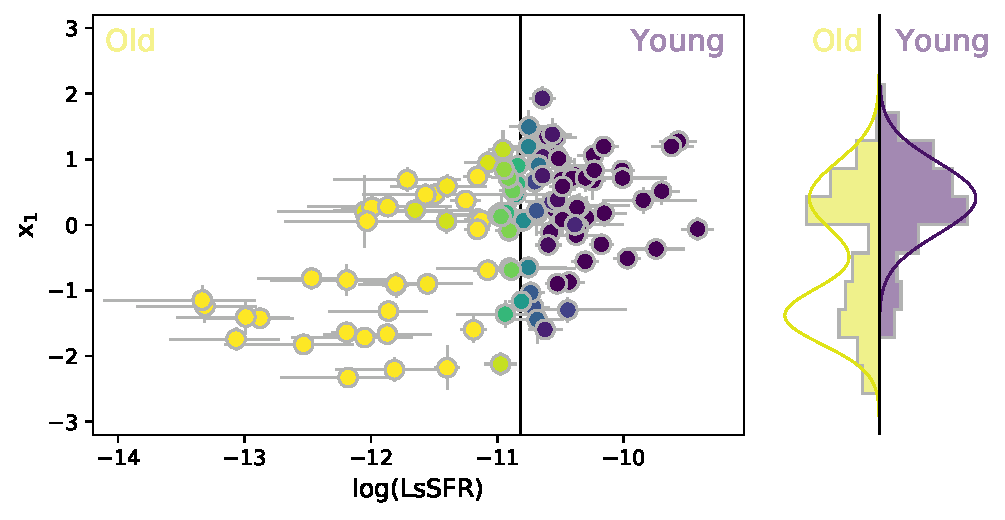
\includegraphics[width=0.8\linewidth]{Article_figures/model_base_hist.pdf}
    \caption{\textit{Main}: \textsc{\texttt{SALT2.4}} lightcurve stretch ($x_1$)
        as a function of the local specific star formation rate (LsSFR) for
        SNfactory SNe used in this analysis. The color corresponds to the
        probability, $p_y$, for the SNe~Ia to be young, i.e. to have
        $\log\mathrm{LsSFR} \geq -10.82$ \citep[see][]{rigault2020}.
        \textit{Right}: $p_y$-weighted histogram of the SN stretches, as well as
        the adjusted Base model; the younger and older population contributions
        are shown in purple and yellow, respectively.}
    \label{fig:stretchlssfr}
\end{figure*}

\begin{itemize}
    \item for the younger population (i.e., $\log(\mathrm{LsSFR})\geq-10.82$),
        the stretch distribution is modeled as a single normal distribution
        $\mathcal{N}(\mu_1, \sigma_1{}^2)$; 
    \item the older population (i.e., $\log( \mathrm{LsSFR})<-10.82$) stretch
        distribution is modeled as a bimodal Gaussian mixture $a\times
        \mathcal{N}(\mu_1, \sigma_1{}^2) + (1-a)\times \mathcal{N}(\mu_2,
        \sigma_2{}^2)$, where one mode is the same as for the young population,
        $a$ representing the relative influence of the two modes.
\end{itemize}

The stretch probability distribution function (pdf) of a given SN will be the
linear combination of the stretch distributions of these two population weighted
by its probability $y^i$ to be young (see Section~\ref{sec:basemodelapplied}).
But generally, the fraction of young SNe~Ia as a function of redshift is given
by $\delta(z)$ (see Eq.~\ref{eq:delta}) and therefore, our redshift drift model
of the underlying distribution of SNe~Ia as a function of redshift $X_1(z)$ is
given by:
\begin{align}\label{eq:stretchz}
    X_1(z) = \delta(z)&\times \mathcal{N}(\mu_1,\sigma_1{}^2) + \nonumber \\
    (1-\delta(z))&\times \left[ a\times\mathcal{N}(\mu_1,\sigma_1{}^2) +
    (1-a)\times\mathcal{N}(\mu_2,\sigma_2{}^2) \right]
\end{align}

\textbf{This is our Base model.}

\subsection{Comparison to data}\label{sec:basemodelapplied}

Given the probability $y^i$ that a given SN is young, and assuming our Base
model (see Section~\ref{sec:basemodel}), the probability to measure a
\textsc{\texttt{SALT2.4}} stretch $x_1^i$ with an error d$x_1^i$ is given by:
\begin{align}\label{eq:likelihoodsnf}
    \prob{x^i_1}{\vec{\theta}; \mathrm{d}x^i_1, y^i} =
    y^i & \times
    \mathcal{N}\left(x^i_1 \mid \mu_1, \sigma_1{}^2+\mathrm{d}x^i_1{}^2\right) +
    \nonumber\\
    (1-y^i) &\times \bigg[
    a \times \mathcal{N}\left(x^i_1 \mid \mu_1,
    \sigma_1{}^2+\mathrm{d}x^i_1{}^2\right) +
    \nonumber\\
    & (1-a) \times \mathcal{N}\left(x^i_1 \mid \mu_2,
    \sigma_2{}^{2}+\mathrm{d}x^i_1{}^2\right) \bigg]
\end{align}

The maximum-likelihood estimate of the 5~free parameters
$\vec{\theta}\equiv({\mu_1,\mu_2,\sigma_1,\sigma_2,a})$ of the model is obtained
by minimizing the following:
\begin{equation}\label{eq:likelihood}
    -2\ln(L) = -2 \sum_i \ln \prob{x_1^i}{\vec{\theta};
    \mathrm{d}x_1^i, y^i}.
\end{equation}

Depending on whether $y^i$ can be estimated directly from LsSFR measurements or
not, there are two ways to proceed, which we now discuss.

\subsubsection{With LsSFR measurements}\label{sec:modelpy}

For the SNfactory sample, we can readily set $y^i = p^i_y$, the probability to
have $\log(\textrm{LsSFR}) \geq -10.82$ (see Fig.~\ref{fig:stretchlssfr}), to
minimize Eq.~\ref{eq:likelihood} with respect to $\vec{\theta}$. Results on
fitting the SNf SNe with this model are shown Table~\ref{tab:modelresults} and
illustrated in Fig.~\ref{fig:modelall}.

\begin{table*}
    \centering
    \caption{Best fit values of the parameters for the Base stretch distribution
    model when applied to the SNfactory dataset only (114 SNe~Ia), the fiducial
569 SN~Ia sample or the conservative one (422).}
    \label{tab:modelresults}
    \begin{tabular}{lccccc}
        \hline\hline
        Sample & $\mu_1$ & $\sigma_1$
               & $\mu_2$ & $\sigma_2$
               & $a$ \\
        \hline
        SNfactory & $ 0.41 \pm 0.08$ & $0.55 \pm 0.06$
                  & $-1.38 \pm 0.10$ & $0.44 \pm 0.08$
                  & $ 0.48 \pm 0.08$ \\
        Fiducial & $ 0.37 \pm 0.05$ & $0.61 \pm 0.04$
                 & $-1.22 \pm 0.16$ & $0.56 \pm 0.10$
                 & $ 0.51 \pm 0.09$ \\
        Conservative & $ 0.38 \pm 0.05$ & $0.60 \pm 0.04$
                     & $-1.26 \pm 0.13$ & $0.53 \pm 0.08$
                     & $ 0.47 \pm 0.09$ \\
        \hline
    \end{tabular}
\end{table*}

\subsubsection{Without LsSFR measurements}\label{sec:modelnopy}

When lacking direct LsSFR measurements (i.e. $p_y^i$), we can extend the
analysis to non-SNfactory samples by using the redshift-evolution of the
fraction $\delta(z)$ of young SNe~Ia (Eq.~\ref{eq:delta}) as a proxy for the
probability of a SN to be young. This still corresponds to minimizing
Eq.~\ref{eq:likelihood} with respect to the parameters
$\vec{\theta}\equiv(\mu_1, \mu_2, \sigma_1, \sigma_2, a)$ of the stretch
distribution $X_1$ (Eq.~\ref{eq:stretchz}), but this time assuming $y^i =
\delta(z^i)$ for any given SN~$i$. 

For the rest of the analysis, we will therefore minimize Eq.~\ref{eq:likelihood}
using $p_y^i$ --~the probability for the SN $i$ to be young~-- when available
(i.e. for SNfactory dataset), and $\delta(z^i)$ --~the expected fraction of
young SNe~Ia at the SN redshift $z^i$~-- otherwise.

Results of fitting this model to all the 569 (resp. 422) SNe from the fiducial
(resp. conservative) sample are given Table~\ref{tab:modelresults}, and the
predicted redshift evolution of mean stretch (expected $x_1$ given the
distribution of Eq.~\ref{eq:stretchz}) illustrated as a blue band in
Fig.~\ref{fig:modelall} accounting for parameters errors and their covariances.
We see in this figure that the measured mean SN~Ia stretch per redshift bins of
equal sample size closely follows our redshift drift modeling. This is indeed
what is expected if old environments favor low SN stretches
\citep[e.g.][]{howell2007} \textit{and} if the fraction of old SNe~Ia declines as
a function of redshift. See Section~\ref{sec:results} for a more quantitative
discussion.

\begin{figure*}
    \centering
    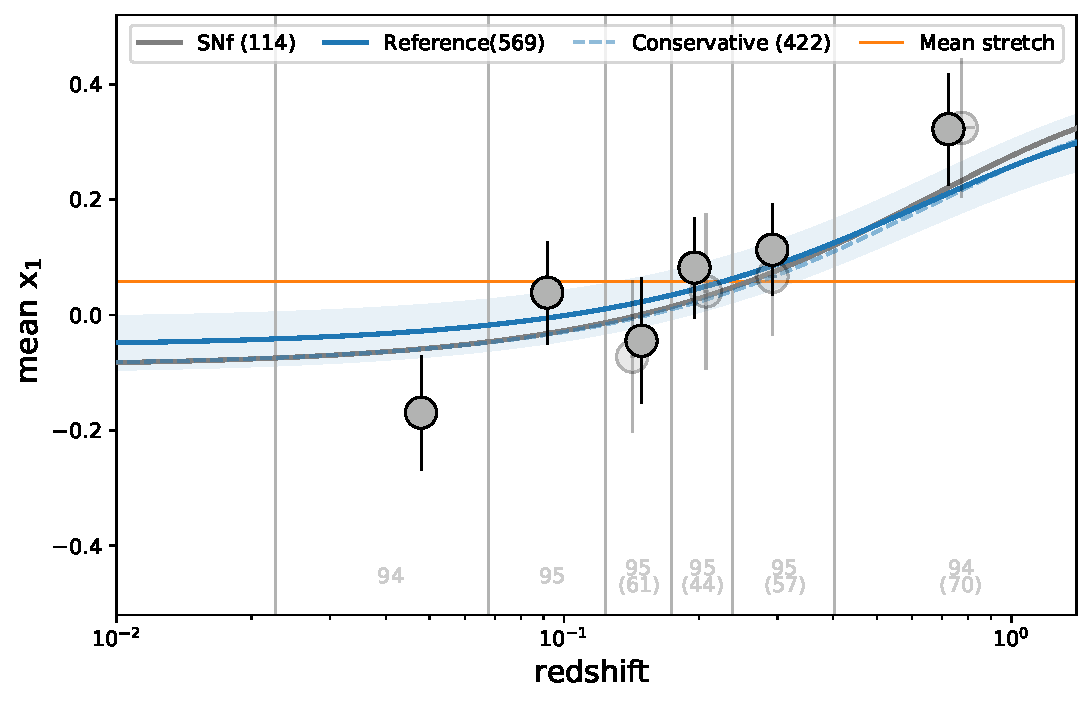
\includegraphics[width=0.7\linewidth]{Article_figures/stretchevol_all_vs_snf-mean.pdf}
    \caption{Evolution of the mean SN \textsc{\texttt{SALT2.4}} stretch ($x_1$)
        as a function of redshift. Markers show the \textbf{stretch plain mean
        (with error estimated from scatter)} measured in redshift bins of equal
        sample size, indicated in light gray at the bottom of each redshift bin.
        Full and light markers are used when considering the fiducial or the
        conservative samples, respectively. The orange horizontal line
        represents the mean stretch \textbf{for the non-evolving Gaussian model
        (last line of Table~\ref{tab:comp}) on the fiducial sample}. Best
        fits of our Base drifting model are shown as blue, dashed-blue and
        gray, when fitted on the fiducial sample, the conservative one or
        the SNfactory dataset only, respectively; all are compatible. The
        light-blue band illustrates the amplitude of the error (incl.
        covariance) of the best fit model when considering the fiducial
    dataset.}
    \label{fig:modelall}
\end{figure*}

\subsection{Alternative models}\label{sec:othermodel}

In Section~\ref{sec:basemodel}, we have modeled the underlying stretch
distribution following \cite{rigault2020}, i.e.\ as a single Gaussian for the
``young'' SNe~Ia and a mixture of two Gaussians for the ``old'' SNe Ia
population, one being the same as for the young population, plus another one for
the fast-declining SNe~Ia that seem to only exist in old local environments.
This is our so-called ``Base'' model. However, to test different modeling
choices, we have implemented a suite of alternative parametrizations that we
also adjust to the data following the procedure described in
Section~\ref{sec:modelnopy}. 

\cite{howell2007} used a simpler unimodal model per age category, assuming a
single normal distribution for each of the young and old populations. We thus
consider a ``Howell+drift'' model, with one single Gaussian per age group and
the $\delta(z)$ drift from Eq.~\ref{eq:delta}.

Alternatively, since we aim at probing the existence of an evolution with
redshift, we also test constant models by restricting the ``Base'' and
``Howell'' models to use a supposedly redshift-independent fraction $\delta(z)
\equiv f$ of young SNe; these models are hereafter labeled ``Base+constant'' and
``Howell+constant''.

We also consider another intrinsically non-drifting model, the functional form
developed for Beams with Bias Correction \cite[BBC,][]{scolnic2016,
kessler2017}, used in recent SN cosmological analyses
\cite[e.g.][]{scolnic2018a, descosmopaper2019, riess2016, riess2019} to account
for Malmquist biases. The BBC formalism assumes sample-based (hence
intrinsically non-drifting) asymmetric Gaussian stretch distributions:
$\mathcal{N}\left(\mu, \sigma_-{}^2\; \text{if} \;x_1<\mu,\; \text{else}
\;\sigma_+{}^2\right)$. The idea behind this sample-based approach is twofold:
(1) Malmquist biases are driven by survey properties and (2) since current
surveys cover limited redshift ranges, having a sample-based approach covers
some potential redshift evolution information \citep{scolnic2016, scolnic2018a}.
See further discussion concerning BBC in Section~\ref{sec:discussion}. 

Finally, for the sake of completeness, we also consider redshift-independent
pure and asymmetric Gaussian models. 

\section{Results}\label{sec:results}

We adjusted each of the models described above on both the fiducial and
conservative samples (cf. Section~\ref{sec:sample}); results are gathered
in Table~\ref{tab:comp}, and illustrated in Fig.~\ref{fig:mod_comp}. 

\begin{table*}
    \centering
    \caption{Comparison of the relative ability of each model to describe the
        data. For each considered model, we report if the model is drifting or
        not, its number of free parameters and, for both the fiducial and the
        conservative cuts, $-2\ln(L)$ (see Eq.~\ref{eq:likelihood}), the AIC and
        the AIC difference ($\Delta$AIC) between this model and the Base model
        used as reference for it has the lowest AIC.}
    \label{tab:comp}
    \begin{tabular}{ccc|ccc|ccc}
        \hline\hline
        & & & \multicolumn{3}{c}{Fiducial sample (569 SNe)}
            & \multicolumn{3}{|c}{Conservative sample (422 SNe)} \\
        Name & drift & $k$ &
        $-2\ln(L)$ & AIC & $\Delta$AIC & $-2\ln(L)$ & AIC & $\Delta$AIC\\
        \hline

        Base & $\delta(z)$ & 5
        & 1456.7 & 1466.7 & -- 
        & 1079.5 & 1089.5 & -- \\

        Howell+drift & $\delta(z)$ & 4
        & 1463.3 & 1471.3 & $-4.6$
        & 1088.2 & 1096.2 & $-6.7$ 
        \\

        Asymmetric & -- & 3
        & 1485.2 & 1491.2 & $-24.5$
        & 1101.3 & 1107.3 & $-17.8$ 
        \\

        Howell+const & $f$ & 5
        & 1484.2 & 1494.2 & $-27.5$
        & 1101.2 & 1111.2 & $-21.7$ 
        \\

        Base+const & $f$ & 6
        & 1484.2 & 1496.2 & $-29.5$
        & 1101.2 & 1113.2 & $-23.7$ 
        \\

        Per sample Asym. & per sample & 3$\times$5
        & 1468.2 & 1498.2 & $-31.5$
        & 1083.6 & 1113.6 & $-24.1$ 
        \\

        Gaussian & -- & 2
        & 1521.8 & 1525.8 & $-59.1$
        & 1142.6 & 1146.6 & $-57.1$ 
        \\
        \hline
    \end{tabular}
\end{table*}

\begin{figure}
    \centering
    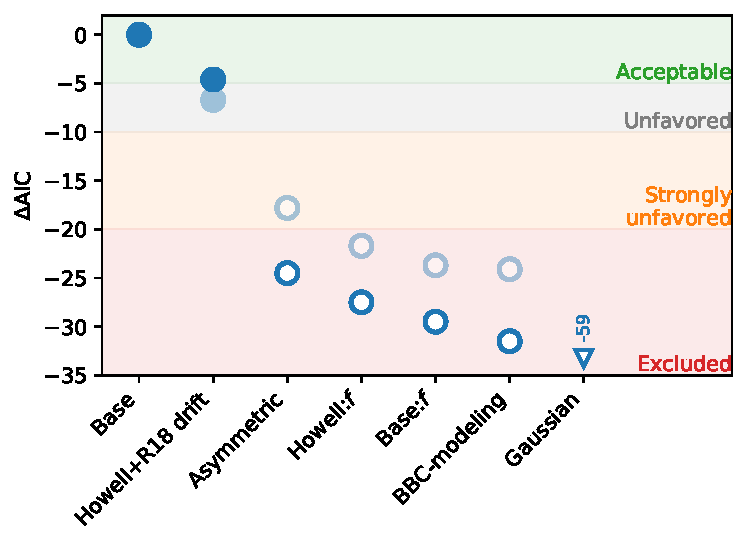
\includegraphics[width=\linewidth]{Article_figures/mod_comp.pdf}
    \caption{$\Delta$AIC between ``Base'' model (reference) and other models
        (see Table~\ref{tab:comp}). Full and open blue markers correspond to
        models with and without redshift drift, respectively. Light markers show
        the results when the analysis is performed on the conservative sample
        rather than the fiducial one. Color-bands illustrate the validity of
        the models, from Acceptable ($\Delta\mathrm{AIC} > -5$) to Excluded
        ($\Delta\mathrm{AIC} < -20$), see text. According to the AIC, all
        non-drifting models (open symbols) are excluded to be as good a
        representation of the data as the Base (drifting) model.}
    \label{fig:mod_comp}
\end{figure}

Since the various models have different degrees of freedom, we use the Akaike
Information Criterion \citep[AIC, e.g.][]{burnham2004} to compare their ability
to properly describe the observations. This estimator penalizes extra degrees of
freedom to avoid over-fitting the data, and is defined as follow:
\begin{equation}
    \mathrm{AIC} = -2\ln(L) + 2k
\end{equation}
where $-2\ln(L)$ is derived by minimizing Eq.~\eqref{eq:likelihood}, and $k$ is
the number of free parameters to be adjusted. The reference model is the one
with the smallest AIC; in comparison to this model, the models with
$\Delta\mathrm{AIC}<5$ are coined acceptable, the ones with
$5<\Delta\mathrm{AIC}<20$ are unfavored, and those with $\Delta\mathrm{AIC}>20$
are deemed excluded. This roughly corresponds to 2, 3 and 5~$\sigma$ limits for
a Gaussian probability distribution. 

The best model (with smallest AIC) is the so-called Base model and thus is our
reference model; this is true both on the fiducial and conservative samples.
The Base model also has the smallest $-2\ln(L)$, making it the most likely
model even ignoring the over-fitting issue accounted for by the AIC formalism.

Furthermore, we find that redshift-independent stretch distributions are all
excluded as suitable descriptions of the data relative to the Base model. In
fact, the best non-drifting model (the Asymmetric one) has a very marginal
chance ($p \equiv \exp\left(\Delta\mathrm{AIC}/2\right) = 5\times10^{-6}$) to
describe the data as well as the Base model. This result is just a quantitative
assessment of qualitative facts clearly visible in Fig.~\ref{fig:modelall}: the
mean SN stretch per bin of redshift strongly suggests a significant redshift
evolution rather than a constant value, and this evolution is well described by
Eq.~\ref{eq:delta}.

Surprisingly, the sample-based Gaussian asymmetric modeling used by current
implementations of the BBC technique \citep{scolnic2016, kessler2017} has one of
the highest AIC value in our analysis (see Section~\ref{sec:results}). While its
$-2\ln(L)$ is the smallest of all redshift-independent models (but still $-11.5$
worse than the reference Base model), it is strongly penalized for requiring
15~free parameters ($\mu_0, \sigma_{\pm}$~for each of the 5~samples of the
analysis). Hence, its $\Delta\mathrm{AIC}<-20$, which could be interpreted as a
probability $p=2\times 10^{-7}$ of being as good a representation of the data
as the Base model.

\textbf{Note} that, when comparing models adjusted on individual subsamples
rather than globally, the Bayesian Information Criterion ($\mathrm{BIC} =
-2\ln(L) + k\ln(n)$, with $n$ the number of data points) might be better suited
than AIC, since it explicitly accounts for the fact that each subsample is
fitted separately: the sample-based model BIC is rightfully the sum of the BIC
for each sample. We find $\Delta\mathrm{BIC}=-48$, again refuting the
sample-based asymmetric Gaussian model as being as pertinent as the Base model.

\textbf{In order to ensure that our results are not driven by the poorly-modeled
    HST sub-sample, we recompute $\Delta$AIC for each model excluding this
    dataset; we find that it does not change $\Delta$AIC by more than few
    tenths. The consistency of these values with those in Table~\ref{tab:comp}
show that the HST sub-sample does not drive our conclusions.}

We report in Table~\ref{tab:bbc} \textbf{our determination of} the samples'
$\mu_0$ and $\sigma_{\pm}$ \textbf{when implementing an asymmetric Gaussian
model}, adjusted on the nominally selection-free samples using our fiducial cuts
(see Section~\ref{sec:sample}). We find our results in close agreement with
\cite{scolnic2016} for SNLS and SDSS and with \cite{scolnic2018a} for PS1, who
derived these model parameters using the full BBC formalism, using numerous
simulations to model the selection effects (see details e.g., Section~3 of
\citealt{kessler2017}). The agreement between our fit of the asymmetric
Gaussians on the supposedly selection-free part of the samples and the results
derived using the BBC formalism supports our approach to \textbf{construct} a
sample with negligible selection effects. If we were to use \cite{scolnic2016}
and \cite{scolnic2018a} best fit values of the $\mu_0, \sigma_{\pm}$ asymmetric
parameters for SNLS, SDSS and PS1, respectively, the $\Delta$AIC between our
Base drifting model and the BBC modeling would go even deeper from $-32$ to
$-47$. We further discuss the consequence of this result for cosmology in
Section~\ref{sec:discussion}.
    
\begin{table}
    \centering
    \caption{Best-fit parameters for our sample-based asymmetric modeling of the
    underlying stretch distribution.}
    \label{tab:bbc}
    \begin{tabular}{ccccccc}
    \hline\hline
    Asymmetric & $\sigma_{-}$ & $\sigma_{+}$ & $\mu_0$ \\
    \hline
    SNfactory & 1.34 $\pm$ 0.13 & 0.41 $\pm$ 0.10 & 0.68 $\pm$ 0.15 \\
    SDSS & 1.31 $\pm$ 0.11 & 0.42 $\pm$ 0.09 & 0.72 $\pm$ 0.13 \\
    PS1 & 1.01 $\pm$ 0.11 & 0.52 $\pm$ 0.12 & 0.38 $\pm$ 0.16 \\
    SNLS & 1.41 $\pm$ 0.13 & 0.15 $\pm$ 0.13 & 1.22 $\pm$ 0.15 \\
    HST & 0.76 $\pm$ 0.36 & 0.79 $\pm$ 0.35 & 0.11 $\pm$ 0.44 \\
    \hline
    \end{tabular}
\end{table}
    
We also performed tests allowing the high-stretch mode of the old population to
differ from the young population mode, hence adding two degrees of freedom. The
corresponding fit is not significantly better, with a $\Delta$AIC of $-0.4$.
This \textbf{reinforces our assumption} that the young and old populations
indeed appear to share the same underlying high-stretch mode. Furthermore, one
might wonder whether a low-stretch mode might also exist in the
young-population, see Fig.~\ref{fig:stretchlssfr}. We \textbf{test for this} by
allowing this population to also be bi-modal, finding the amplitude of
\textbf{such a} low-stretch mode to be compatible with~0 in this young
population ($<2\%$). More generally, this raises the question of \textbf{how
well a given environmental tracer (here LsSFR) traces the age}. A dedicated
analysis will be presented in Briday et al.\ in prep.

Finally, ignoring the LsSFR measurements --~available only for the SNfactory
dataset, see Section~\ref{sec:modeling}~-- reduces the significance of the
results presented in this section, as expected. Yet, non-drifting models remain
strongly disfavored, and for instance, the best fitted sample-based Gaussian
asymmetric modeling still is $\Delta\mathrm{AIC}<-10$ less representative of the
data than our Base drifting modeling.

\section{Discussion}\label{sec:discussion}

To the best of our knowledge, a SN~Ia stretch redshift drift modeling has never
been explicitly used in cosmological analyses, though Bayesian hierarchy
formalism such as UNITY \citep{rubin2015}, BAHAMAS \citep{shariff2016} or Steve
\citep{hinton2019} can easily allow it; see e.g., section 1.3 and 2.5 of
\cite{rubin2015}. Not doing so is a second order issue for SN cosmology, as it
only affects the way one accounts for Malmquist bias. Indeed, as long as the
Phillips relation \citep{phillips1993} standardization parameter $\alpha$ is not
redshift dependent (a study \textbf{beyond} the scope of this paper, but see
e.g. \citealt{scolnic2018a}), the stretch-corrected SNe~Ia magnitudes used for
cosmology are blind to the underlying stretch distribution for complete samples.
However, surveys usually do have significant Malmquist bias for the upper half
of their SN redshift distribution. As a consequence, an ill-modeling of the
underlying stretch distribution will bias the SN magnitudes derived from such
surveys. 

Commonly used Malmquist bias correction techniques, such as the BBC-formalism,
assume per sample asymmetric Gaussian functions for modeling the underlying
stretch and color distributions. Yet, as shown in Section~\ref{sec:results},
such a sample-based distribution is excluded as being as good as our drifting
model. Then, unlike what \citet[][Section~2]{scolnic2016} and
\citet[][Section~5.4]{scolnic2018a} suggested, i.e. that traditional surveys
span limited redshift ranges and that therefore the per-sample approach accounts
for implicit redshift drifts, a direct modeling of the redshift drift is more
appropriate than a sample-based approach. We \textbf{add} here that, as
measurements of modern surveys try to cover increasingly larger redshift ranges
in order to reduce calibration systematic uncertainties, this sample-based
approach \textbf{becomes} less valid, notably for PS1, DES and, soon, LSST.

We illustrate in Fig.~\ref{fig:bbc_pdf_ps1} the prediction difference in the
underlying stretch distribution between the per-sample asymmetric modeling and
our Base drifting model for the PS1 sample. Our model is bimodal and the
relative amplitude of each mode depends on the redshift-dependent fraction of
old and young SNe~Ia in the sample: the higher the fraction of old SNe~Ia (at
lower redshift), the higher the amplitude of the old-specific low-stretch mode.
This redshift dependency is shown as blue to red underlying distributions in
Fig.~\ref{fig:bbc_pdf_ps1} for redshift ranges covered by PS1. The observed
$x_1$ histogram follows \textbf{the model we defined using} the sum of
individual underlying SN-redshift distributions. As expected, the two modeling
approaches differ mostly in the negative part of the SN stretch distribution.
The asymmetric Gaussian distribution goes through the middle of the bimodal
distribution, over-estimating the number of SNe~Ia at $x_1\sim-0.7$ and
under-estimating it at $x_1\sim-1.7$ in comparison to our Base drifting model
for typical PS1 SN redshifts. This means that the SN bias-corrected standardized
magnitude estimated at a redshift affected by selection effects would be biased
by an ill-modeling of the true underlying stretch distribution.

\begin{figure}
    \centering
    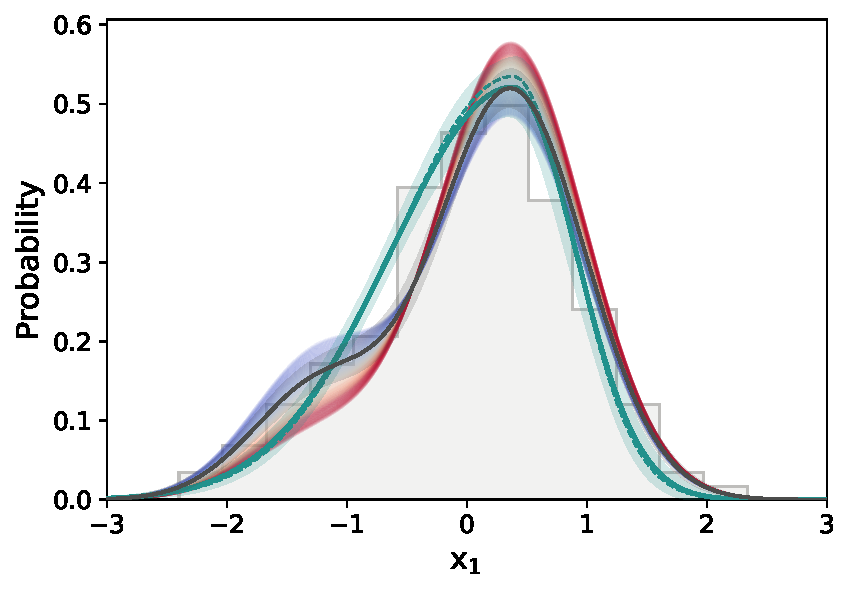
\includegraphics[width=\linewidth]{Article_figures/bbc_comp_PS1_hist-nr.pdf}
    \caption{Distribution of the PS1 SN~Ia \textsc{\texttt{SALT2.4}} stretch
        ($x_1$) after the fiducial redshift limit cut (grey histogram). This
        distribution is supposed to be a random draw from the underlying stretch
        distribution. The green lines show the BBC model of this underlying
        distribution (asymmetric Gaussian). The full line (band) is our best fit
        (its error); the dashed line shows the \cite{scolnic2018a} result. The
        black line (band) shows our best fitted Base-modeling (its error, see
        Table \ref{tab:modelresults}) that includes redshift drift. For
        illustration, we show as colored (from blue to red with increasing
        redshifts) the evolution of the underlying stretch distribution as a
        function of redshift for the redshift range covered by PS1 data.}
    \label{fig:bbc_pdf_ps1}
\end{figure}

\textbf{Assessing t}he amplitude of this magnitude bias for cosmology is beyond
the scope of this paper given the complexity of the BBC analysis. It would
require a full study using our Base model (Eq.~\ref{eq:stretchz}) in place of
the sample-based asymmetric modeling as part of the BBC simulations. However, we
already highlight that even if a non-drifting sample-based model could provide
comparable result in the volume-limited part of the various samples, these
models would differ when extrapolating to higher redshifts, precisely where the
underlying distribution will matter for correcting Malmquist biases.

In the era of modern cosmology, where we aim \textbf{to measure} $w_0$ at a
sub-percent level and $w_a$ \textbf{with} ten-percent precision
\citep[e.g.,][]{lsstpaper}, we stress that correct modeling of potential SN
redshift drift should be further studied and care should be taken when using
samples affected by selection effects.

\section{Conclusion}\label{sec:ccl}

We have presented \textbf{an initial} study of the drift of the underlying SNe~Ia
stretch distribution as a function of redshift. We built a magnitude-limited
SN~Ia sample from the Pantheon dataset \citep[][SDSS, PS1 and
SNLS]{scolnic2018a}, to which we added HST and SNfactory data from
\cite{rigault2020} for the high- and low-redshift bins. We only considered the
SNe that have been discovered in the redshift range of each survey where
selection effects are negligible, so that the observed SNe~Ia stretches are
a random sampling of the true underlying distribution. This resulted in a 569
SN~Ia fiducial sample (422 SNe when more conservative cuts were considered).

Following predictions made in \cite{rigault2020}, we introduced a redshift drift
model which depends on the expected fraction of ``young'' and ``old'' SNe~Ia as
a function of redshift, \textbf{with} each age population having its own
underlying stretch distribution.

In addition to this ``base'' modeling, we have studied various distributions,
including redshift independent models; we also studied the prediction from a
per-sample asymmetric Gaussian stretch distribution used, for instance, by the
Beams with Bias Correction Malmquist bias correction algorithm
\citep{scolnic2016, kessler2017}.

Our conclusions are the following:
\begin{enumerate}
    \item The underlying SN~Ia stretch distribution is significantly redshift
        dependent, as previously suggested by e.g.~\cite{howell2007}, \textbf{in
        a way that selection effects alone cannot explain}. This result is
        largely independent of details on each age-population model.
    
    \item Redshift-independent models are \textbf{quantitatively} excluded as
        suitable descriptions of the data relative to our Base model. This model
        assumes that: (1) the younger population has a unimodal Gaussian stretch
        distribution, while the older population stretch distribution is
        bimodal, one mode being the same as the young one; (2) the evolution of
        the relative fraction of younger and older SNe~Ia follows the prediction
        made in \cite{rigault2020}. This second result strongly supports the
        existence of both young and old SN~Ia populations, in agreement with
        rate studies \cite{mannucci2005, scannapieco2005, sullivan2006,
        aubourg2008}. 
        
    \item Models using survey-based asymmetric Gaussian distributions, as done,
        e.g., in the current implementation of BBC, are excluded \textbf{as a}
        good description of the data relative to our drifting model. Hence, the
        sample-based approach does not accurately account for redshift drift and
        even less so as survey span increasingly larger redshift ranges.
        \textbf{As a result, if} extra degrees of freedom might be acceptable
        given the large number of SNe~Ia in cosmological studies, extrapolating
        the SN property distributions from the volume-limited part of a survey
        to its Malmquist-biased magnitude-limited one would still be inaccurate
        because of the redshift evolution.

    \item Given the current dataset, we suggest the use of the following stretch
        population model as a function of redshift:
        \begin{align*}
        \label{eqconclusion:stretchz}
            X_1\left(z \right) =
            \delta(z)&\times\mathcal{N}(\mu_1,\sigma_1{}^2)\,+\nonumber\\
            (1-\delta(z))&\times \left[a\times\mathcal{N}(\mu_1,\sigma_1{}^2) +
            (1-a)\times\mathcal{N}(\mu_2,\sigma_2{}^2)\right]
            \tag{\ref{eq:stretchz}}
        \end{align*}
        with $a=0.51$, $\mu_1=0.37$, $\mu_2=-1.22$, $\sigma_1=0.61$,
        $\sigma_2=0.56$ (see Table~\ref{tab:modelresults}), and using the
        age-population drift model \begin{align*}
            \delta(z) & = \left( K^{-1} \times (1+z)^{-2.8} +1 \right)^{-1}
            \tag{\ref{eq:delta}}
        \end{align*}
        with $K=0.87$.
\end{enumerate}

In this paper, we considered a simple \textbf{two-population} Gaussian mixture
modeling, but additional data free from significant Malmquist bias would enable
us to refine it as necessary. We note that samples at the low- and high-redshift
ends of the Hubble diagram would be particularly helpful for this drifting
analysis; fortunately this will soon be provided by the Zwicky Transient
Facility \citep[low-$z$,][]{bellm2019, graham2019}, and Subaru and SeeChange
SNe~Ia programs (high-$z$), respectively. 

\textbf{The next step of the analysis will be to incorporate our modeling within
the SNANA framework \citep{SNANA} both to more accurately account for selection
functions and to test the impact of our modeling on the derivation of
cosmological parameters; this study is underway.}

\begin{acknowledgements}
    This project has received funding from the European Research Council (ERC)
    under the European Union's Horizon 2020 Research and Innovation program
    (grant agreement no 759194 - USNAC).
    This work was supported in part by the Director, Office of Science, Office
    of High Energy Physics of the U.S. Department of Energy under Contract No.
    DE-AC025CH11231.
    This project is partly financially supported by Région Rhône-Alpes-Auvergne.
\end{acknowledgements}

\bibliographystyle{aa}
\begin{thebibliography}{} 
% A

\bibitem[Abbott et al.(2019)]{descosmopaper2019} Abbott, T.~M.~C., Allam, S.,
Andersen, P., et al.\ 2019, \apjl, 872, L30

\bibitem[Aldering et al.(2002)]{aldering2002} Aldering, G., Adam, G., Antilogus,
P., et al.\ 2002, \procspie, 61

\bibitem[Aldering et al.(2020)]{aldering2020} Aldering, G., Antilogus, P.,
Aragon, C., et al.\ 2020, Research Notes of the American Astronomical Society,
4, 63

\bibitem[Astier et al.(2006)]{astier2006} Astier, P., Guy, J., Regnault, N., et
al.\ 2006, \aap, 447, 31

\bibitem[Aubourg et al.(2008)]{aubourg2008} Aubourg, {\'E}., Tojeiro, R.,
Jimenez, R., et al.\ 2008, \aap, 492, 631 

% B

\bibitem[Bazin et al.(2011)]{bazin2011} Bazin, G., Ruhlmann-Kleider, V.,
Palanque-Delabrouille, N., et al.\ 2011, \aap, 534, A43

\bibitem[Bellm et al.(2019)]{bellm2019} Bellm, E.~C., Kulkarni, S.~R., Graham,
M.~J., et al.\ 2019, \pasp, 131, 018002

\bibitem[Betoule et al.(2014)]{betoule2014} Betoule, M., Kessler, R., Guy, J.,
et al.\ 2014, \aap, 568, A22

\bibitem[Brout et al.(2019)]{brout2019} Brout, D., Scolnic, D., Kessler, R., et
al.\ 2019, \apj, 874, 150

\bibitem[Burnham \& Anderson(2004)]{burnham2004} Burnham, K., Anderson, D., \
2004, Sociological Methods \& Research, 33, 2

% C

\bibitem[Campbell et al.(2013)]{campbell2013} Campbell, H., D'Andrea, C.~B.,
Nichol, R.~C., et al.\ 2013, \apj, 763, 88

\bibitem[Childress et al.(2013)]{childress2013} Childress, M., Aldering, G.,
Antilogus, P., et al.\ 2013, \apj, 770, 108

\bibitem[Childress et al.(2014)]{childress2014} Childress, M.~J., Wolf, C., \&
Zahid, H.~J.\ 2014, \mnras, 445, 1898

% D

\bibitem[D'Andrea et al.(2011)]{dandrea2011} D'Andrea, C.~B., Gupta, R.~R.,
Sako, M., et al.\ 2011, \apj, 743, 172

\bibitem[Dilday et al.(2008)]{dilday2008} Dilday, B., Kessler, R., Frieman,
J.~A., et al.\ 2008, \apj, 682, 262

% E
% F

\bibitem[Feeney et al.(2019)]{feeney2019} Feeney, S.~M., Peiris, H.~V.,
Williamson, A.~R., et al.\ 2019, \prl, 122, 061105

\bibitem[Freedman et al.(2019)]{freedman2019} Freedman, W.~L., Madore, B.~F.,
Hatt, D., et al.\ 2019, \apj, 882, 34

\bibitem[Freedman et al.(2020)]{freedman2020} Freedman, W.~L., Madore, B.~F.,
Hoyt, T., et al.\ 2020, \apj, 891, 57. doi:10.3847/1538-4357/ab7339

\bibitem[Frieman et al.(2008)]{frieman2008} Frieman, J.~A., Bassett, B., Becker,
A., et al.\ 2008, \aj, 135, 338

% G

\bibitem[Graham et al.(2019)]{graham2019} Graham, M.~J., Kulkarni, S.~R., Bellm,
E.~C., et al.\ 2019, \pasp, 131, 078001

\bibitem[Gupta et al.(2011)]{gupta2011} Gupta, R.~R., D'Andrea, C.~B., Sako, M.,
et al.\ 2011, \apj, 740, 92

\bibitem[Guy et al.(2007)]{guy2007} Guy, J., Astier, P., Baumont, S., et al.\
2007, \aap, 466, 11

% H

\bibitem[Hamuy et al.(1996)]{hamuy1996} Hamuy, M., Phillips, M.~M., Suntzeff,
N.~B., et al.\ 1996, \aj, 112, 2391

\bibitem[Hamuy et al.(2000)]{hamuy2000} Hamuy, M., Trager, S.~C., Pinto, P.~A.,
et al.\ 2000, \aj, 120, 1479

\bibitem[Hinton et al.(2019)]{hinton2019} Hinton, S.~R., Davis, T.~M., Kim,
A.~G., et al.\ 2019, \apj, 876, 15

\bibitem[Howell et al.(2007)]{howell2007} Howell, D.~A., Sullivan, M., Conley,
A., et al.\ 2007, \apjl, 667, L37

% I

\bibitem[Ivezi{\'c} et al.(2019)]{lsstpaper} Ivezi{\'c}, {\v{Z}}., Kahn, S.~M.,
Tyson, J.~A., et al.\ 2019, \apj, 873, 111

% J

\bibitem[Jones et al.(2015)]{jones2015} Jones, D.~O., Riess, A.~G., \& Scolnic,
D.~M.\ 2015, \apj, 812, 3 1

\bibitem[Jones et al.(2018)]{jones2018} Jones, D.~O., Riess, A.~G., Scolnic,
D.~M., et al.\ 2018, \apj, 867, 108

\bibitem[Jones et al.(2018)b]{jones2018b} Jones, D.~O., Scolnic, D.~M., Riess,
A.~G., et al.\ 2018, \apj, 857, 51

\bibitem[Jones et al.(2019)]{jones2019} Jones, D.~O., Scolnic, D.~M., Foley,
R.~J., et al.\ 2019, \apj, 881, 19

% K

\bibitem[Kelly et al.(2010)]{kelly2010} Kelly, P.~L., Hicken, M., Burke, D.~L.,
et al.\ 2010, \apj, 715, 743

\bibitem[Kessler et al.(2009)]{kessler2009} Kessler, R., Becker, A.~C., Cinabro,
D., et al.\ 2009, \apjs, 185, 32

\bibitem[Kessler et al.(2009)]{SNANA} Kessler, R., Bernstein, J.~P., Cinabro,
D., et al.\ 2009, \pasp, 121, 1028

\bibitem[Kessler \& Scolnic(2017)]{kessler2017} Kessler, R., \& Scolnic, D.\
2017, \apj, 836, 56

\bibitem[Kim et al.(2018)]{kim18} Kim, Y.-L., Smith, M., Sullivan, M., et al.\
2018, \apj, 854, 24

\bibitem[Kim et al.(2019)]{kim19} Kim, Y.-L., Kang, Y., \& Lee, Y.-W.\ 2019,
Journal of Korean Astronomical Society, 52, 181

\bibitem[Knox \& Millea(2020)]{knox2019} Knox, L. \& Millea, M.\ 2020, \prd,
101, 043533. doi:10.1103/PhysRevD.101.043533

% L

\bibitem[Lampeitl et al.(2010)]{lampeitl2010} Lampeitl, H., Smith, M., Nichol,
R.~C., et al.\ 2010, \apj, 722, 566

% M

\bibitem[Mannucci et al.(2005)]{mannucci2005} Mannucci, F., Della Valle, M.,
Panagia, N., et al.\ 2005, \aap, 433, 807 

\bibitem[Mannucci et al.(2006)]{mannucci2006} Mannucci, F., Della Valle, M., \&
Panagia, N.\ 2006, \mnras, 370, 773 

\bibitem[Maoz et al.(2014)]{maozmannucci2014} Maoz, D., Mannucci, F., \&
Nelemans, G.\ 2014, \araa, 52, 107 


% N

\bibitem[Neill et al.(2006)]{neill2006} Neill, J.~D., Sullivan, M., Balam, D.,
et al.\ 2006, \aj, 132, 1126

\bibitem[Neill et al.(2009)]{neill2009} Neill, J.~D., Sullivan, M., Howell,
D.~A., et al.\ 2009, \apj, 707, 1449

\bibitem[Nordin et al.(2018)]{nordin2018} Nordin, J., Aldering, G., Antilogus,
P., et al.\ 2018, \aap, 614, A71

% O
% P

\bibitem[Pan et al.(2014)]{pan2014} Pan, Y.-C., Sullivan, M., Maguire, K., et
al.\ 2014, \mnras, 438, 1391

\bibitem[Perlmutter et al.(1999)]{perlmutter1999} Perlmutter, S., Aldering, G.,
Goldhaber, G., et al.\ 1999, \apj, 517, 565

\bibitem[Perrett et al.(2010)]{perrett2010} Perrett, K., Balam, D., Sullivan,
M., et al.\ 2010, \aj, 140, 518

\bibitem[Phillips(1993)]{phillips1993} Phillips, M.~M.\ 1993, \apjl, 413, L105

\bibitem[Planck Collaboration et al.(2020)]{planck2018} Planck
Collaboration, Aghanim, N., Akrami, Y., et al.\ 2020, \aap, 641, A6.
doi:10.1051/0004-6361/201833910

\bibitem[Poulin et al.(2019)]{poulin2019} Poulin, V., Smith, T.~L., Karwal, T.,
et al.\ 2019, \prl, 122, 221301

% Q
% R

\bibitem[Reid et al.(2019)]{reid2019} Reid, M.~J., Pesce, D.~W., \& Riess,
A.~G.\ 2019, \apjl, 886, L27. doi:10.3847/2041-8213/ab552d

\bibitem[Rest et al.(2014)]{rest2014} Rest, A., Scolnic, D., Foley, R.~J., et
al.\ 2014, \apj, 795, 44

\bibitem[Riess et al.(1998)]{riess1998} Riess, A.~G., Filippenko, A.~V.,
Challis, P., et al.\ 1998, \aj, 116, 1009

\bibitem[Riess et al.(2009)]{riess2009} Riess, A.~G., Macri, L., Casertano, S.,
et al.\ 2009, \apj, 699, 539

\bibitem[Riess et al.(2016)]{riess2016} Riess, A.~G., Macri, L.~M., Hoffmann,
S.~L., et al.\ 2016, \apj, 826, 56

\bibitem[Riess et al.(2018)]{riess2018} Riess, A.~G., Casertano, S., Yuan, W.,
et al.\ 2018, \apj, 861, 126

\bibitem[Riess et al.(2019)]{riess2019} Riess, A.~G., Casertano, S., Yuan, W.,
et al.\ 2019, \apj, 876, 85

\bibitem[{Rigault {et~al.}(2013)}]{rigault2013} Rigault, M., Copin, Y.,
Aldering, G., {et~al.} 2013, \aap, 560, A66

\bibitem[Rigault et al.(2015)]{rigault2015} Rigault, M., Aldering, G., Kowalski,
M., et al.\ 2015, \apj, 802, 20

\bibitem[Rigault et al.(2020)]{rigault2020} Rigault, M., Brinnel, V., Aldering,
G., et al.\ 2029, \aap, 644, A176

\bibitem[Rodney et al.(2014)]{rodney2014} Rodney, S.~A., Riess, A.~G., Strolger,
L.-G., et al.\ 2014, \aj, 148, 13 
  
\bibitem[Roman et al.(2018)]{roman2018} Roman, M., Hardin, D., Betoule, M., et
al.\ 2018, \aap, 615, A68

\bibitem[Rose et al.(2019)]{rose2019} Rose, B.~M., Garnavich, P.~M., \& Berg,
M.~A.\ 2019, \apj, 874, 32

\bibitem[Rubin et al.(2015)]{rubin2015} Rubin, D., Aldering, G., Barbary, K., et
al.\ 2015, \apj, 813, 137

\bibitem[Rubin \& Hayden(2016)]{rubin2016} Rubin, D., \& Hayden, B.\ 2016,
\apjl, 833, L30

% S

\bibitem[Sako et al.(2008)]{sako2008} Sako, M., Bassett, B., Becker, A., et al.\
2008, \aj, 135, 348

\bibitem[Saunders et al.(2020)]{saunders2020} Saunders, C., Aldering, G.,
Antilogus, P., et al.\ 2020, VizieR Online Data Catalog, J/ApJ/869/167

\bibitem[Scannapieco \& Bildsten(2005)]{scannapieco2005} Scannapieco, E., \&
Bildsten, L.\ 2005, \apjl, 629, L85 

\bibitem[Scolnic et al.(2014)]{scolnic2014} Scolnic, D., Rest, A., Riess, A., et
al.\ 2014, \apj, 795, 45

\bibitem[Scolnic \& Kessler(2016)]{scolnic2016} Scolnic, D., \& Kessler, R.\
2016, \apjl, 822, L35

\bibitem[Scolnic et al.(2018)]{scolnic2018a} Scolnic, D.~M., Jones, D.~O., Rest,
A., et al.\ 2018a, \apj, 859, 101

\bibitem[Scolnic et al.(2019)]{scolnicastro2020} Scolnic, D., Perlmutter, S.,
Aldering, G., et al.\ 2019, Astro2020: Decadal Survey on Astronomy and
Astrophysics, 2020, 270

\bibitem[Shariff et al.(2016)]{shariff2016} Shariff, H., Jiao, X., Trotta, R.,
et al.\ 2016, \apj, 827, 1

\bibitem[Strolger et al.(2004)]{strolger04} Strolger, L.-G., Riess, A.~G.,
Dahlen, T., et al.\ 2004, \apj, 613, 200

\bibitem[Sullivan et al.(2006)]{sullivan2006} Sullivan, M., Le Borgne, D.,
Pritchet, C.~J., et al.\ 2006, \apj, 648, 868 

\bibitem[Sullivan et al.(2010)]{sullivan2010} Sullivan, M., Conley, A., Howell,
D.~A., et al.\ 2010, \mnras, 406, 782

% T

\bibitem[Tasca et al.(2015)]{tasca2015} Tasca, L.~A.~M., Le F{\`e}vre, O.,
Hathi, N.~P., et al.\ 2015, \aap, 581, A54

% U 
% V
% W

\bibitem[Wiseman et al.(2020)]{wiseman2020} Wiseman, P., Smith, M., Childress,
M., et al.\ 2020, \mnras, 495, 4040. doi:10.1093/mnras/staa1302

\bibitem[Wong et al.(2020)]{wong2019} Wong, K.~C., Suyu, S.~H., Chen, G.~C.-F.,
et al.\ 2020, \mnras, 498, 1420. doi:10.1093/mnras/stz3094

% X
% Y
% Z
\end{thebibliography}
\end{document}
